\documentclass{article}

% - Style
\usepackage{base}

% - Plotting
\usepgfplotslibrary{units}
\usepackage{pgfplotstable}

% - Listings
\usepackage{color}
\usepackage{listings}

\lstset{
  basicstyle=\ttfamily\footnotesize\color{black}
  , commentstyle=\color{blue}
  , keywordstyle=\color{purple}
  , stringstyle=\color{orange}
  %
  , numbers=left
  , numbersep=5pt
  , stepnumber=1
  , numberstyle=\ttfamily\small\color{black}
  %
  , keepspaces=true
  , showspaces=false
  , showstringspaces=false
  , showtabs=false
  , tabsize=2
  , breaklines=true
  %
  , frame=single
  , backgroundcolor=\color{white}
  , rulecolor=\color{black}
  , captionpos=b
}

% file or folder
\lstdefinestyle{ff}{
  basicstyle=\ttfamily\normalsize\color{orange}
}

% - Title
\title{PHYS4004 High Performance Computing - Assignment 2: MPI}
\author{Tom Ross - 1834 2884}
\date{}

% - Headers
\pagestyle{fancy}
\fancyhf{}
\rhead{\theauthor}
\chead{}
\lhead{\thetitle}
\rfoot{\thepage}
\cfoot{}
\lfoot{}

% - Document
\begin{document}

\tableofcontents

\newpage
\section{Overview}
\label{sec:overview}

The codebase \lstinline[style=ff]{mandelbrot}, which can be found at
\url{https://github.com/dgsaf/mandelbrot}, consists of the original code
provided by Associate Professor Nigel Marks, with the following additions:
\begin{itemize}
\item \lstinline[style=ff]{src/mandelbrot_static.f90}:

\item \lstinline[style=ff]{src/mandelbrot_master_worker.f90}:

\item \lstinline[style=ff]{src/mandelbrot_cyclic.f90}:

\item \lstinline[style=ff]{mandelbrot.slurm}:

\item \lstinline[style=ff]{mandelbrot-static.slurm}:

\item \lstinline[style=ff]{mandelbrot-master_worker.slurm}:

\item \lstinline[style=ff]{mandelbrot-cyclic.slurm}:

\item \lstinline[style=ff]{mandelbrot-jobs.sh}:

\item \lstinline[style=ff]{output/}:

\item \lstinline[style=ff]{bin/}:

\item \lstinline[style=ff]{pictures/}:

\end{itemize}

\newpage
\section{Serial}
\label{sec:serial}

The Mandelbrot serial code, \lstinline[style=ff]{src/mandelbrot.f90}, can be
found in \autoref{sec:serial-code}.

\newpage
\section{Static Decomposition}
\label{sec:static}

The Mandelbrot MPI static decomposition code,
\lstinline[style=ff]{src/mandelbrot_static.f90}, can be found in
\autoref{sec:static-code}.

% compare performance with serial code

% discuss load balance

% load balance graph
The load-balance for the 10 processes is show in
\autoref{fig:static-load-balance}.
\begin{figure}[h]
  \centering
  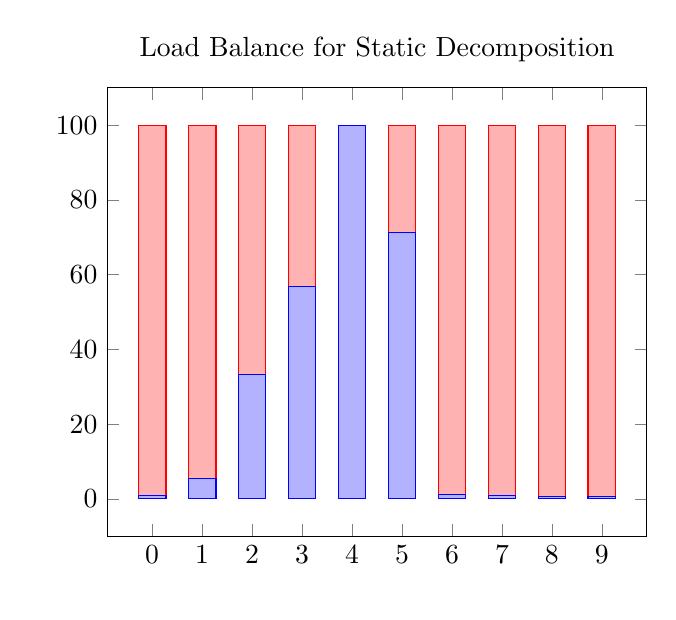
\begin{tikzpicture}
    \pgfplotstableread[col sep=comma, header=true]{
      process, working, waiting, communicating
      0,  0.91, 98.94, 0.15
      1,  5.42, 94.54, 0.03
      2, 33.25, 66.70, 0.05
      3, 56.85, 43.09, 0.06
      4, 99.92,  0.00, 0.08
      5, 71.39, 28.52, 0.09
      6,  1.21, 98.68, 0.11
      7,  0.78, 99.10, 0.12
      8,  0.68, 99.18, 0.14
      9,  0.60, 99.25, 0.15
    }\data

    \begin{axis}[
      ybar stacked
      , xtick={0, 1, ..., 9}
      , ymin=-10
      , ymax=110
      , ytick={0, 20, ..., 100}
      , title={Load Balance for Static Decomposition}
      ]

      \addplot table[x=process, y=working] from \data;
      \addplot table[x=process, y=waiting] from \data;
      \addplot table[x=process, y=communicating] from \data;

    \end{axis}
  \end{tikzpicture}
  \caption{The load balance for the Mandelbrot MPI static decomposition scheme,
    with 10 processes, where $N = 8000$, $\mathrm{maxiter} = 1000$. For each
    process, the percentage of time spent working is shown in blue, the
    percentage of time spent waiting in red, and the percentage of time spent
    communicating is shown in brown (however, this time is negligble and so is
    barely visible).}
  \label{fig:static-load-balance}
\end{figure}

\newpage
\section{Master-Worker Scheme}
\label{sec:master-worker}

The Mandelbrot MPI master-worker scheme code,
\lstinline[style=ff]{src/mandelbrot_master_worker.f90}, can be
found in \autoref{sec:master-worker-code}.

% compare performance with static

% compare load balance with static (for chunksize = 100000)
The load-balance for the 9 worker processes is show in
\autoref{fig:master-load-balance}.
\begin{figure}[h]
  \centering
  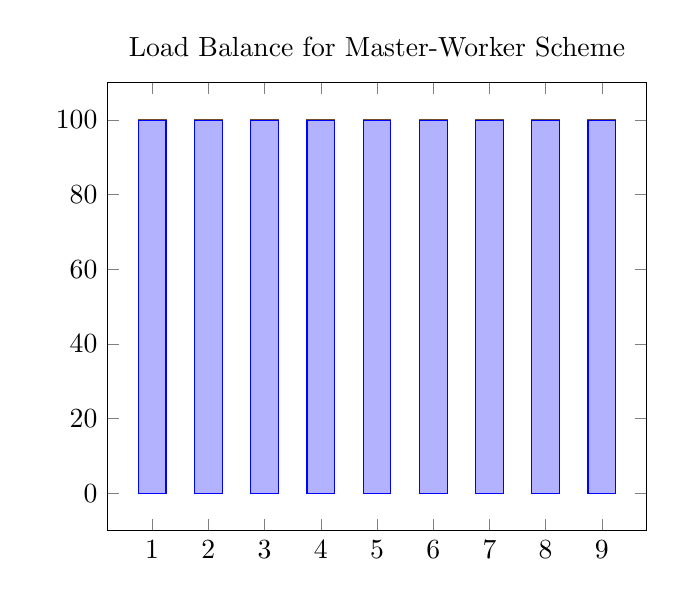
\begin{tikzpicture}
    \pgfplotstableread[col sep=comma, header=true]{
      process, working, waiting, communicating
      1, 99.80, 0.00, 0.20
      2, 99.83, 0.00, 0.17
      3, 99.81, 0.00, 0.19
      4, 99.80, 0.00, 0.20
      5, 99.80, 0.00, 0.20
      6, 99.80, 0.00, 0.20
      7, 99.78, 0.00, 0.22
      8, 99.82, 0.00, 0.18
      9, 99.79, 0.00, 0.21
    }\data

    \begin{axis}[
      ybar stacked
      , xtick={0, 1, ..., 9}
      , ymin=-10
      , ymax=110
      , ytick={0, 20, ..., 100}
      , title={Load Balance for Master-Worker Scheme}
      ]

      \addplot table[x=process, y=working] from \data;
      \addplot table[x=process, y=waiting] from \data;
      \addplot table[x=process, y=communicating] from \data;

    \end{axis}
  \end{tikzpicture}
  \caption{The load balance for the Mandelbrot MPI master-worker scheme,
    with 10 processes, where $N = 8000$, $\mathrm{maxiter} = 1000$, and
    $\mathrm{chunksize} = 100000$. For each worker process, the percentage of
    time spent working is shown in blue, the percentage of time spent waiting in
    red, and the percentage of time spent communicating is shown in brown;
    however, the time spent waiting and communicating is negligble and so both
    are barely visible.}
  \label{fig:master-load-balance}
\end{figure}

% discuss how load balance varies with chunksize

% execution time graph vs chunksize
The time taken for the Mandelbrot MPI master-worker scheme to terminate for
varying chunk sizes is shown in \autoref{fig:scaling-chunksize}.
\begin{figure}[h]
  \centering
  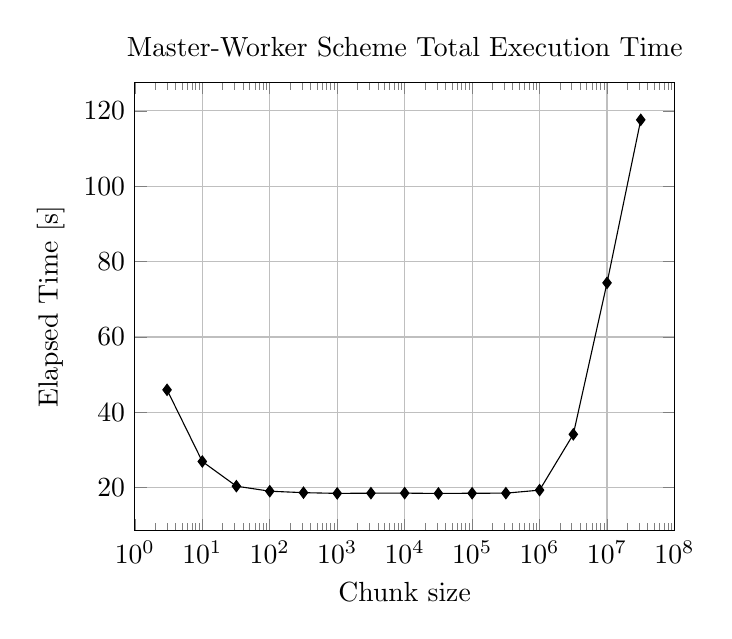
\begin{tikzpicture}
    \pgfplotstableread[col sep=comma, header=true]{
      chunksize, elapsedtime
      3, 45.985
      10, 26.966
      32, 20.422
      100, 19.087
      316, 18.700
      1000, 18.512
      3162, 18.560
      10000, 18.577
      31623, 18.492
      100000, 18.548
      316228, 18.569
      1000000, 19.368
      3162278, 34.179
      10000000, 74.364
      31622777, 117.62
    }\data

    \begin{axis}[
      use units
      , title = {Master-Worker Scheme Total Execution Time}
      , grid = major
      , xmode = log
      , log basis x = {10}
      , xlabel = {Chunk size}
      , ylabel = {Elapsed Time}
      , y unit = {s}
      , xmin = 1
      , xmax = 100000000
      ]

      \addplot [
      color = black
      , mark = diamond*
      ] table [x=chunksize, y=elapsedtime] \data;

    \end{axis}
  \end{tikzpicture}
  \caption{The total execution time for the Mandelbrot MPI master-worker scheme,
  with 10 processes, where $N=8000$, $\mathrm{maxiter}=1000$, for a range of
  chunk sizes, $\mathrm{chunksize} = 10^{k/2}$ for $k = 1, \dotsc, 15$. The MPI
  master-worker scheme, for a chunk size of $1$, failed to terminate within
  10 minutes and so was disregarded.}
  \label{fig:scaling-chunksize}
\end{figure}

\clearpage
\section{Cyclic Decomposition}
\label{sec:cyclic}

The Mandelbrot MPI cyclic decomposition code,
\lstinline[style=ff]{src/mandelbrot_cyclic.f90}, can be found in
\autoref{sec:cyclic-code}.

% compare performance with static

% discuss load imbalance
The load-balance for the 10 worker processes is show in
\autoref{fig:cyclic-load-balance}.
\begin{figure}[h]
  \centering
  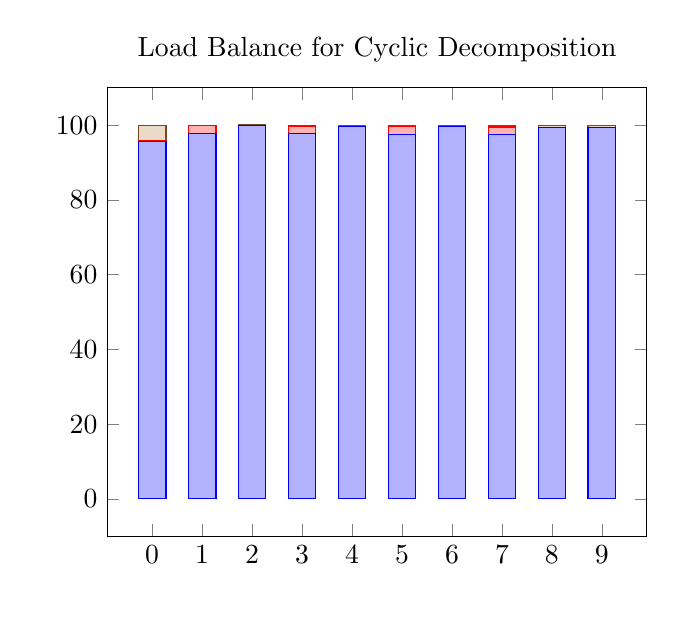
\begin{tikzpicture}
    \pgfplotstableread[col sep=comma, header=true]{
      process, working, waiting, communicating
      0, 95.76, 0.18, 4.06
      1, 97.86, 2.06, 0.08
      2, 99.86, 0.08, 0.13
      3, 97.74, 2.06, 0.20
      4, 99.67, 0.07, 0.26
      5, 97.61, 2.06, 0.33
      6, 99.55, 0.07, 0.38
      7, 97.49, 2.05, 0.46
      8, 99.41, 0.07, 0.51
      9, 99.30, 0.08, 0.62
    }\data

    \begin{axis}[
      ybar stacked
      , xtick={0, 1, ..., 9}
      , ymin=-10
      , ymax=110
      , ytick={0, 20, ..., 100}
      , title={Load Balance for Cyclic Decomposition}
      ]

      \addplot table[x=process, y=working] from \data;
      \addplot table[x=process, y=waiting] from \data;
      \addplot table[x=process, y=communicating] from \data;

    \end{axis}
  \end{tikzpicture}
  \caption{The load balance for the Mandelbrot MPI cyclic decomposition scheme,
    with 10 processes, where $N = 8000$, $\mathrm{maxiter} = 1000$. For each
    worker process, the percentage of time spent working is shown in blue, the
    percentage of time spent waiting in red, and the percentage of time spent
    communicating is shown in brown. It can be seen that the only process with
    non-negligble communication time is the root thread. This is due to the time
    spent re-ordering the cyclic data gathered at the root thread into the
    original sequential order being included in the time spent communicating for
    the root process. This was chosen since while cyclic decomposition may have
    benefits, untangling the returned data is a significant consideration.}
  \label{fig:cyclic-load-balance}
\end{figure}

% discuss which is best strategy

\clearpage
\appendix
\section{Appendix}
\label{sec:appendix}

\subsection{Serial}
\label{sec:serial-code}

\lstinputlisting[
language=Fortran
]{../src/mandelbrot.f90}

\newpage
\subsection{Static Decomposition}
\label{sec:static-code}

\lstinputlisting[
language=Fortran
]{../src/mandelbrot_static.f90}

\newpage
\subsection{Master Worker Scheme}
\label{sec:master-worker-code}

\lstinputlisting[
language=Fortran
]{../src/mandelbrot_master_worker.f90}

\newpage
\subsection{Cyclic Decomposition}
\label{sec:cyclic-code}

\lstinputlisting[
language=Fortran
]{../src/mandelbrot_cyclic.f90}


\end{document}